% !TeX spellcheck = en_US
% !TeX encoding = UTF-8
% !TeX program = xelatex

\documentclass[12pt]{article}
\usepackage[left=2cm, right=2cm, top=2cm, bottom=2cm]{geometry}
\usepackage{float}

\usepackage{bbm}
\usepackage{fontspec}
\usepackage{polyglossia} 
\usepackage{amsmath,amsfonts,amssymb,amsthm,mathtools}
\usepackage{amsmath}
\usepackage{stmaryrd}
\usepackage{bm}
\usepackage{graphicx}
\usepackage{subcaption}
\usepackage{bbm}
\usepackage{enumitem}
%\usepackage{enumerate}
\usepackage[bookmarks=false]{hyperref}

\usepackage{fancyvrb}

\usepackage{adjustbox}

% \usepackage{csquotes}
% \usepackage[backend=biber, style=apa, autocite=inline]{biblatex}
% \addbibresource{bibl.bib} 

% \usepackage{natbib}

\setsansfont{Linux Biolinum O}
\setromanfont{Linux Biolinum O} 
\setmonofont[Mapping=tex-text]{Courier New}

\usepackage{xcolor}
\usepackage{soul}

\setdefaultlanguage{english}

\newcommand{\N}{\mathbb{N}}
\newcommand{\Z}{\mathbb{Z}}
\newcommand{\E}{\mathbb{E}}
\DeclareMathOperator{\corr}{\mathop{corr}}
\DeclareMathOperator{\Corr}{\mathop{Corr}}
\DeclareMathOperator{\cov}{\mathop{cov}}
\DeclareMathOperator{\Cov}{\mathop{Cov}}
\DeclareMathOperator{\var}{\mathop{var}}
\DeclareMathOperator{\Var}{\mathop{Var}}
\DeclareMathOperator{\tr}{\mathop{tr}}
\DeclareMathOperator{\diag}{\mathop{diag}}
\DeclareMathOperator{\plim}{\mathop{plim}}
\DeclareMathOperator{\mmod}{\mathop{mod}}

\newcommand{\toD}{\stackrel{d}{\longrightarrow}}
\newcommand{\toP}{\stackrel{p}{\longrightarrow}}
\newcommand{\norm}[1]{\left\lVert#1\right\rVert}
\newcommand{\approxtext}[1]{\ensuremath{\stackrel{\text{#1}}{\sim}}}
\newcommand{\?}{\stackrel{?}{=}}
\renewcommand{\epsilon}{\varepsilon}
\renewcommand{\phi}{\varphi}

\mathtoolsset{showonlyrefs=true}

\usepackage{pgffor,newfile}
\newcommand*{\conoptprb}[4][\max]{%
    \newoutputstream{constraints}
    \openoutputfile{\jobname.constraints}{constraints}
    \foreach \entry [count=\ni] in {#4}
    {
        \ifnum\ni=1
            \addtostream{constraints}{& \text{  s.t.} & & \entry \\}
        \else
            \addtostream{constraints}{& & & \entry \\}
        \fi
    }
    \closeoutputstream{constraints}

  \begin{equation}
  \begin{aligned}
  & \underset{#2}{#1} & & #3 \\
  \input{\jobname.constraints}
  \end{aligned}
  \end{equation}
}


\begin{document}
\title{\vspace{-1.5cm} Advanced Topics in Macroeconomics 1. Problem Set 1}
\author{Evgenii Ivanov \and Walter Verwer}
\date{November 5, 2021}
 
\maketitle

\section*{Problem 1}

\subsection*{(a) Solve the model by value function iteration.}
Solving the model via value function iteration gives us the results displayed in figures \ref{fig:pol} and \ref{fig:val}.
\begin{figure}[htbp!]
    \centering
    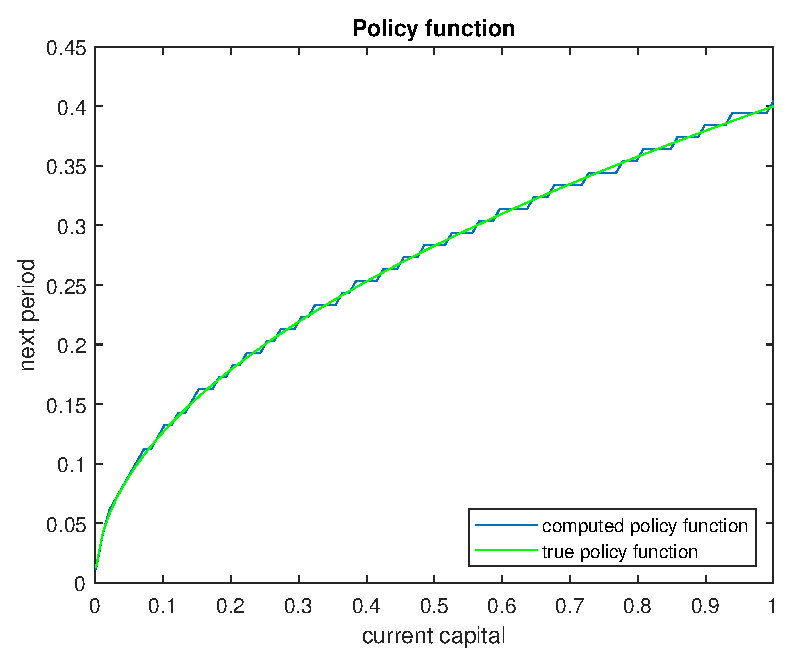
\includegraphics[width=0.45\textwidth]{PS1/1_Policy_Function_without.eps}
    \caption{Policy function using the brute-force method. Parameters: $\delta=1$, $\beta=0.96$, and $\alpha=0.3$.}
    \label{fig:pol}
\end{figure}

\begin{figure}[htbp!]
    \centering
    \includegraphics[width=0.45\textwidth]{PS1/1_Value_function_without.eps}
    \caption{Value function using the brute-force method. Parameters: $\delta=1$, $\beta=0.96$, and $\alpha=0.3$.}
    \label{fig:val}
\end{figure}

\begin{table}[htbp!]
    \centering
    \begin{tabular}{c|c|c}
         Method & Time (sec) & Number of iterations \\
         \hline
         Brute-force & 0.177915 & 395 \\
         Monotonicity & 0.179421 & 395 \\
         Concavity & 0.206627 & 395 \\
         Howard's pol. & 0.013470 & 18
    \end{tabular}
    \caption{Performance for the different methods. Parameters: $\delta=1$, $\beta=0.96$, and $\alpha=0.3$.}
    \label{tab:res}
\end{table}

\subsection*{(b) Exploit monotonicity of the policy function and evaluate its performance.}
In table \ref{tab:res} we have displayed the four different methods to compute the value function. We observe that exploiting monotonicity

\subsection*{(c) Exploit concavity of the value function and evaluate its performance.}
Looking at table \ref{tab:res}, we observe

\subsection*{(d) Code Howard's policy iteration and evaluate its performance.}
Looking at table \ref{tab:res} again, we know observe a large increase in performance, compared to the other methods.




\section*{Problem 2}

Firstly let us derive the expression for the steady state level of capital.

The value function is:

\[
V(K) = \max_{k'} [ u(zf(k) + (1-\delta)k - k') + \beta V(k')]
\]

The first order condition:

\[
-u_c (c) + \beta V(k') = 0
\]
where $c = zf(k) + (1-\delta)k - k'$

The envelope condition:

\[
V'(k) = u_c (c) (zf'(k) + 1-\delta)
\]

Therefore if we combine them together we get the Euler equation:

\[
u_c (c) = \beta u_c (c') (zf'(k') + 1-\delta) 
\]

In the steady state $k'=k=k^*$ and $c$ is also constant:

\[
1 = \beta (zf'(k^*) + 1 - \delta)
\]
\[
f'(k^*) = z^{-1} \left( \frac{1}{\beta} - 1 + \delta \right)
\]

If we assume $f(k) = k^\alpha$ then $f'(k) = \alpha k^{\alpha-1}$ and then the steady state capital level is:

\[
k^* = \left[ \frac{1}{\alpha z} \left( \frac{1}{\beta} - 1 + \delta \right) \right]^{\frac{1}{\alpha-1}}
\]

\section*{Problem 3}

\section*{Problem 4}

The rate of convergence of the Bisection method is linear and slow but it is guaranteed to converge if function is real and continuous in an interval bounded by given two initial guess.
Accuracy of bisection method is very good and this method is more reliable than other open methods like Secant, Newton Raphson method etc.

Despite being slower to converge, accuracy of this method increases as number of iterations increases.

In Bisection method, error is reduced by factor of ½ after each iterations, so we can write: en+1/en = 1/2. Which gives:

en+1 = en/2

Or, en+1 = 0.5 en ----- (1)

Here en+1 is error at n+1th iteration and en is error at nth iteration.

From equation (1) it can be concluded that, error at n+1th iteration is linearly related to error at nth iteration i.e. en+1 ∝ en

For this reason, Bisection method is said to have linear rate of convergence.



\end{document}